\documentclass{article}

% if you need to pass options to natbib, use, e.g.:
%     \PassOptionsToPackage{numbers, compress}{natbib}
% before loading neurips_2020

% ready for submission
% \usepackage{neurips_2020}

% to compile a preprint version, e.g., for submission to arXiv, add add the
% [preprint] option:
    %   \usepackage[preprint]{neurips_2020}

% to compile a camera-ready version, add the [final] option, e.g.:
       \usepackage[final]{neurips_2020}

% to avoid loading the natbib package, add option nonatbib:

    % \usepackage[nonatbib]{neurips_2020}


\usepackage[utf8]{inputenc} % allow utf-8 input
\usepackage[T1]{fontenc}    % use 8-bit T1 fonts
\usepackage{hyperref}       % hyperlinks
\usepackage{url}            % simple URL typesetting
\usepackage{booktabs}       % professional-quality tables
\usepackage{amsfonts}       % blackboard math symbols
\usepackage{nicefrac}       % compact symbols for 1/2, etc.
\usepackage{microtype}      % microtypography
\usepackage{authblk}
\usepackage{graphicx}

\title{NNTI-2021 FINAL NLP PROJECT REPORT \newline 		HINDI/BENGALI SENTIMENT ANALYSIS}


\author{
  Shahrukh Khan\\
  \texttt{shkh00001@uni-saarland.de}\\
  \textbf{matriculation number 7003144}
  \and
  Mahnoor Shahid\\
  \texttt{mash00001@uni-saarland.de}\\
  \textbf{matriculation number 7003144}
}

\begin{document}

\maketitle


\begin{abstract}
 This part of report is abstract. Lorem ipsum dolor sit amet, consetetur sadipscing elitr, sed diam nonumy eirmod tempor invidunt ut labore et dolore magna aliquyam erat, sed diam voluptua. At vero eos et accusam et justo duo dolores et ea rebum. Stet clita kasd gubergren, no sea takimata sanctus est Lorem ipsum dolor sit amet.
\end{abstract}

\textbf{Keywords}
\begin{list}
    \item -Deep Learning, Pytorch, NLP, Sentiment Analysis, Hate Speech
\end{list}


\section{Submission of NNTI Final Project 2021}

NLP task was selected. Bleh bleh bleh bleh. Below you can find the link to the project repository. 
\begin{center}
  \url{https://github.com/shahrukhx01/nnti_hindi_bengali_sentiment_analysis}
\end{center}

\section{Task One: Word Embeddings}
\label{gen_inst}

Lorem ipsum dolor sit amet, consetetur sadipscing elitr, sed diam nonumy eirmod tempor invidunt ut labore et dolore magna aliquyam erat, sed diam voluptua. At vero eos et accusam et justo duo dolores et ea rebum. Stet clita kasd gubergren, no sea takimata sanctus est Lorem ipsum dolor sit amet.

\section{Influence of Hashtags and Emojis on Sentiment Analysis of the datasets: Hindi and Bengali }
\label{headings}

In general, the usage of hashtags in a sentence can benefit us in investigation under many various aspects, one of the common ones that includes Context Identification, Sentiment Analyses etc. Mostly, there is great influence of hashtags on the sentences:

\begin{itemize}
    \item As just by observing the words that are used as hashtags or by perceiving the high volumes of certain hashtags can direct us to the subject of the content or the trending topic. 
   \item Correspondingly, it can affect the strength of the sentiment in a sentence, for example multiple negative hashtags can increase the negative sentiment of a tweet.
\end{itemize}

For these certain reasons we have settled not to eliminate them. 

Our dataset is consisting of tweets in the targeted languages; Hindi and Bengali, and these text sentences are provided to us, marked already with the flags: HOF and NOT [1] as shown in Table 1 so we will be using these indicators to segregate whether the hashtags belong to a negative sentence or non-negative sentence, to know how much proportion of hate speech our dataset has.

\begin{table}

  \caption{Flags marked on Hindi Dataset and their meanings}
  \label{Table 3.0}
  \centering
  \begin{tabular}{cl}
    \toprule                \
    Flag     & What it means \\
    \midrule
    HOF (Hate and Offensive)     & Tweets that contains hate, offensive and aggressive words are \\ & labeled using this \\
    NOT (Non Hate-Offensive)     & Tweets that has no indication of any hate and offensive words are \\ & labeled using this.  \\
    \bottomrule
  \end{tabular}
\end{table}


\subsection{Dividing the tweets into negative vs non-negative sentences}

Before we have extracted the hashtags from the dataset, we have divided the data based on the flags \textbf{HOF} and \textbf{NOT}, so that we can get to know the proportion of negative and non-negative text sentences in our provided Hindi Dataset. As shown in Table 1, we can perceive that our dataset has almost equal ratio of negative and non-negative sentences. 

\begin{table}[b]
\begin{center}
  \caption{Tweets divided into Negative vs NonNegative Sentences}
  \centering
  \begin{tabular}{p{2cm}  l p{2cm} }
    \toprule                \
    Flag     & No. of Sentences     & Proportion \\
    \midrule
    HOF     & 2469   & 52.92\% \\
    NOT     & 2196   & 47.07\%  \\
    \bottomrule
  \end{tabular}
\end{center}
\end{table}


\subsection{Extracting the hashtags from Hindi Dataset}
Once we have separated the data frames, we will extract the hashtags out of our dataset for further investigation. We have then used the matcher class from the spacy package (python library) to match the sequences of the tokens, based on pattern rules and obtained the hash tags for both the negative and non-negative sentences.

\subsection{Examining the proportion of hashtags}

For better understanding of the proportion of the hashtags that we have obtained from our Hindi dataset, we will visualize the tags in the pie chart. As can be distinguished in the Figure 1, there is a remarkable difference between the hashtags we have for negative sentences in the comparison to the non-negative. We only have a total of \textbf{25.4\%}  of the hashtags from the negative sentences in our entire Hindi dataset.

\begin{figure}
  \centering
  
  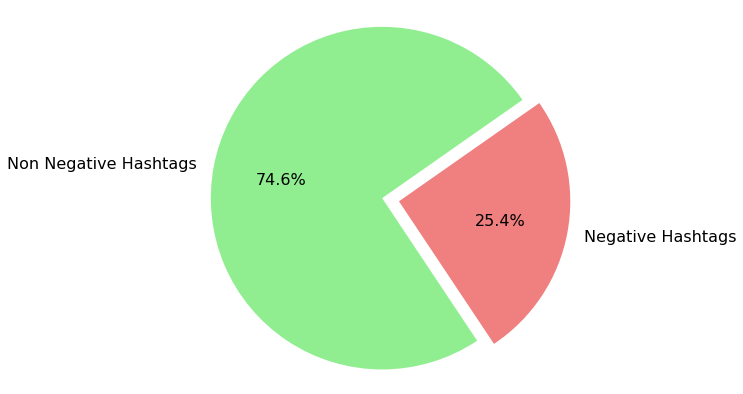
\includegraphics[width=10.2cm, height=5.5cm]{piechart.png}
%   \fbox{\rule[-.5cm]{0cm}{4cm} \rule[-.5cm]{4cm}{0cm}}
  \caption{Hastags in Hindi Dataset for Negative vs Non-Negative Sentences}
\end{figure}

\subsection{Investigating the sentiment of hashtags}

In order to extract the sentiment of the words used for hashtags, we have used TextBlob module imported from textblob (python library), since we can observe that all the hashtags in the Hindi Dataset are english alphabetic words. \textit{Subsequently, we have found 0 polarity for all the hash tags, meaning they do not provide any assistance or they have no impact in the positive and negative sentiment of sentence.} However, the frequency of a particular hashtag or the frequency of related hashtags can led us to know about the topic of the tweets. So we will further look into the frequency count.

\subsection{Detecting the content of the hashtags}

If the purpose of the study is based on the context of subject or the topic of the tweets, then these hashtags in the Hindi Dataset tells us much more about that. Figure 2 is an example wordcloud that represents the most used words as the hashtags in the Hindi Dataset, where blue hashtags represent the ones used in negative sentences and the grey hashtags represent the ones used in positive sentences, interestingly, from which we can spot that even though the proportion of the Negative Hashtags was one-fourth in contrast to Non-Negative hashtags, the most frequent hashtags were the negative ones and the topics on which we will have the hate-speech are the tweets mostly regarding politics and cricket matches.

\begin{figure}[b]
  \centering
  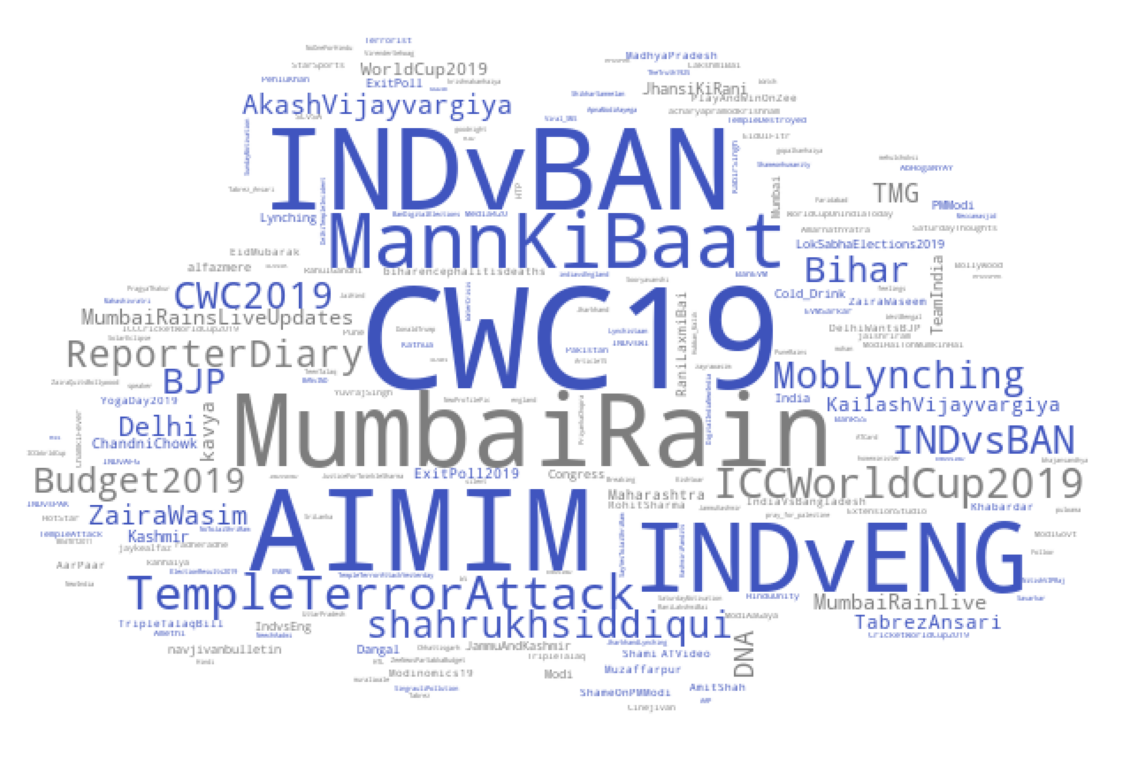
\includegraphics[width=13cm, height=7cm]{wordcloud2.png}
%   \fbox{\rule[-.5cm]{0cm}{4cm} \rule[-.5cm]{4cm}{0cm}}
  \caption{WordCloud indicating the most frequent hashtags in the Hindi Dataset}
\end{figure}

\subsection{Further exploration for the emojis}

With the intention to obtain the emojis from the Hindi Dataset we have used Regex and have specified all the Emoji Unicode Blocks in the pattern and have used the findall() method to get the list of emojis, regrettably we have just 2 emojis in the entire dataset. \textit{So, removing them and not removing them will not make any difference in this setting.  }



\section{Analysis on the Word2Vec Model created in Task One}
\label{others}

By setting different values for Hyperparameters with different combinations, this was observed that for the better performance of the model's parameters should be set to Epochs=500, Window Size=1, Embedded Size=300, Batch Size=8, Learning Rate=0.05


\subsection{Finding the better Batch Size for the model with Window Size = 1}



The documentation for \verb+natbib+ may be found at
\begin{center}
  \url{http://mirrors.ctan.org/macros/latex/contrib/natbib/natnotes.pdf}
\end{center}
Of note is the command \verb+\citet+, which produces citations appropriate for
use in inline text.  For example,
\begin{verbatim}
   \citet{hasselmo} investigated\dots
\end{verbatim}
produces
\begin{quote}
  Hasselmo, et al.\ (1995) investigated\dots
\end{quote}

If you wish to load the \verb+natbib+ package with options, you may add the
following before loading the \verb+neurips_2020+ package:
\begin{verbatim}
   \PassOptionsToPackage{options}{natbib}
\end{verbatim}

If \verb+natbib+ clashes with another package you load, you can add the optional
argument \verb+nonatbib+ when loading the style file:
\begin{verbatim}
   \usepackage[nonatbib]{neurips_2020}
\end{verbatim}

As submission is double blind, refer to your own published work in the third
person. That is, use ``In the previous work of Jones et al.\ [4],'' not ``In our
previous work [4].'' If you cite your other papers that are not widely available
(e.g., a journal paper under review), use anonymous author names in the
citation, e.g., an author of the form ``A.\ Anonymous.''

\subsection{Footnotes}

Footnotes should be used sparingly.  If you do require a footnote, indicate
footnotes with a number\footnote{Sample of the first footnote.} in the
text. Place the footnotes at the bottom of the page on which they appear.
Precede the footnote with a horizontal rule of 2~inches (12~picas).

Note that footnotes are properly typeset \emph{after} punctuation
marks.\footnote{As in this example.}

\subsection{Figures}

\begin{figure}
  \centering
  \fbox{\rule[-.5cm]{0cm}{4cm} \rule[-.5cm]{4cm}{0cm}}
  \caption{Sample figure caption.}
\end{figure}

All artwork must be neat, clean, and legible. Lines should be dark enough for
purposes of reproduction. The figure number and caption always appear after the
figure. Place one line space before the figure caption and one line space after
the figure. The figure caption should be lower case (except for first word and
proper nouns); figures are numbered consecutively.

You may use color figures.  However, it is best for the figure captions and the
paper body to be legible if the paper is printed in either black/white or in
color.

\subsection{Tables}

All tables must be centered, neat, clean and legible.  The table number and
title always appear before the table.  See Table~\ref{sample-table}.

Place one line space before the table title, one line space after the
table title, and one line space after the table. The table title must
be lower case (except for first word and proper nouns); tables are
numbered consecutively.

Note that publication-quality tables \emph{do not contain vertical rules.} We
strongly suggest the use of the \verb+booktabs+ package, which allows for
typesetting high-quality, professional tables:
\begin{center}
  \url{https://www.ctan.org/pkg/booktabs}
\end{center}
This package was used to typeset Table~\ref{sample-table}.

\begin{table}
  \caption{Sample table title}
  \label{sample-table}
  \centering
  \begin{tabular}{lll}
    \toprule
    \multicolumn{2}{c}{Part}                   \\
    \cmidrule(r){1-2}
    Name     & Description     & Size ($\mu$m) \\
    \midrule
    Dendrite & Input terminal  & $\sim$100     \\
    Axon     & Output terminal & $\sim$10      \\
    Soma     & Cell body       & up to $10^6$  \\
    \bottomrule
  \end{tabular}
\end{table}

\section{Summary}

Lorem ipsum dolor sit amet, consetetur sadipscing elitr, sed diam nonumy eirmod tempor invidunt ut labore et dolore magna aliquyam erat, sed diam voluptua. At vero eos et accusam et justo duo dolores et ea rebum. Stet clita kasd gubergren, no sea takimata sanctus est Lorem ipsum dolor sit amet.

\section*{References}

References follow the acknowledgments. Use unnumbered first-level heading for
the references. Any choice of citation style is acceptable as long as you are
consistent. It is permissible to reduce the font size to \verb+small+ (9 point)
when listing the references.
{\bf Note that the Reference section does not count towards the eight pages of content that are allowed.}
\medskip

\small

[1] Thomas Mandl, Sandip Modha, Prasenjit Majumder, Daksh Patel, Mohana Dave, Chintak Mandlia, and Aditya Patel. Overview of the hasoc track at fire 2019: Hate speech and offensive content identification in indo-european languages. In Proceedings of the 11th Forum for Information Retrieval Evaluation, pages 14–17, 2019.


\end{document}